\documentclass[10pt,a4paper]{article}
\usepackage[utf8]{inputenc}
\usepackage[spanish]{babel}
\usepackage{amsmath}
\usepackage{amsfonts}
\usepackage{amssymb}
\usepackage{float}
\usepackage{graphicx}
\usepackage[left=2cm,right=2cm,top=2cm,bottom=2cm]{geometry}
\author{Lisandro Alvarez}
\title{Informe Parte 3}
\begin{document}
\section{Parte 3}
Se pidió desarrollar un programa con interfaz gráfica de usuario, cuyo propósito fuera el de facilitar la confección de gráficos, mediante un método de ploteo automático. El programa debe implementarse en Python, y debe cumplir con los siguientes requisitos básicos. 
En primer lugar, respecto a fuentes desde las cuales se puede ingresar datos a graficar, los mismos deben ser:
\begin{itemize}
\item Función transferencia
\item Archivo LTspice
\item Plantilla de Excel o csv con mediciones
\end{itemize}
En segundo lugar, se de debe otorgar al usuario las siguientes capacidades:
\begin{itemize}
\item Especificar la etiqueta para el eje x.
\item Especificar la etiqueta para el eje y.
\item Guardar el gráfico como imagen.
\item Borrar todos los gráficos anteriores.
\item Graficar más de tres señales simultáneamente.
\end{itemize}

\subsection{Guía de usuario}
A continuación se explicará detalladamente cada paso referente a la utilización de la GUI implementada. Los pasos a desarrollar son el ingreso de datos desde los distintos tipos de fuentes, edición de las etiquetas, seleccionar la visualización del gráfico en una o dos figuras, eliminar los gráficos anteriores y por ultimo, la exportación de los gráficos.

Previo a desarrollar los pasos se muestra una figura con el diseño de la interfaz gráfica, tal cual se muestra una vez que el usuario inicia el programa

\begin{figure}[ht]
\centering
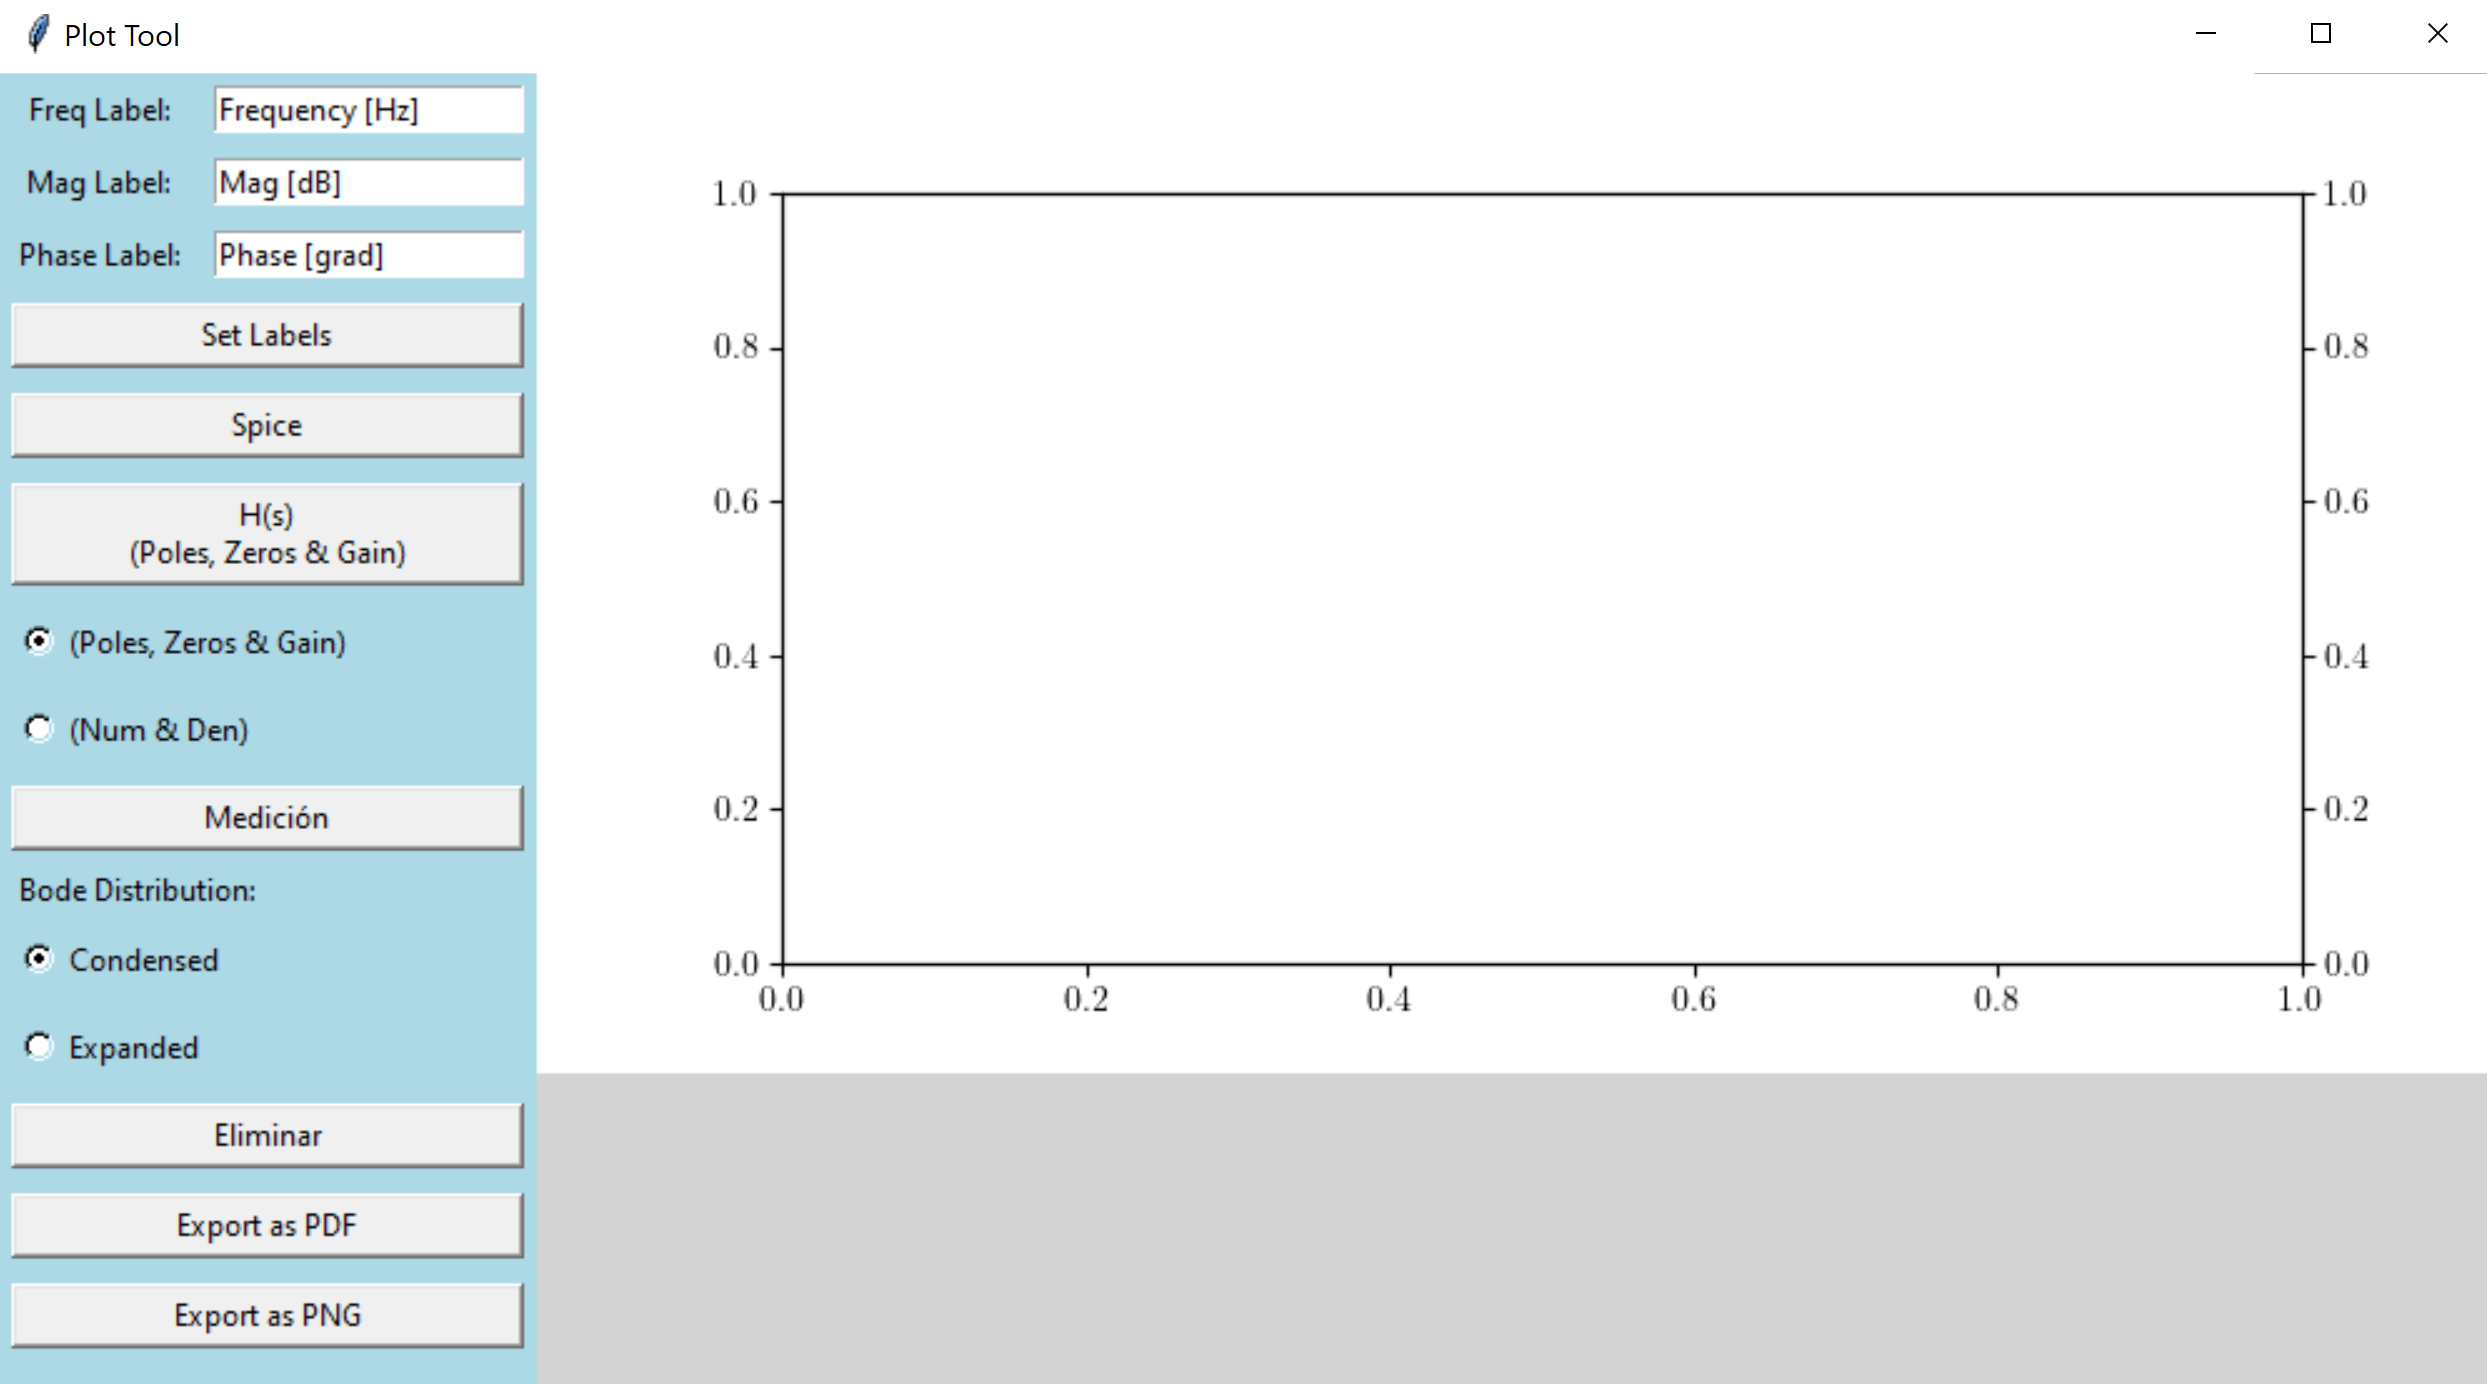
\includegraphics[scale=0.2]{window.png}
\caption{GUI al iniciar el programa}
\label{fig:window}
\end{figure}

A la izquierda se encuentra el panel de controles, cuyo funcionamiento se explicara a continuación, mientras que a la derecha se encuentra la figura donde se graficarán nuestros datos.

\subsubsection{Ingresar datos}
El programa nos permite ingresar datos desde tres fuentes distintas, archivos de LTspice, transferencias analíticas o mediciones(en un formato determinado que se explicara posteriormente). Las tres opciones están presentes en la GUI referenciadas en la Figura\ref{fig:controlPanel}

\begin{figure}[ht]
\centering
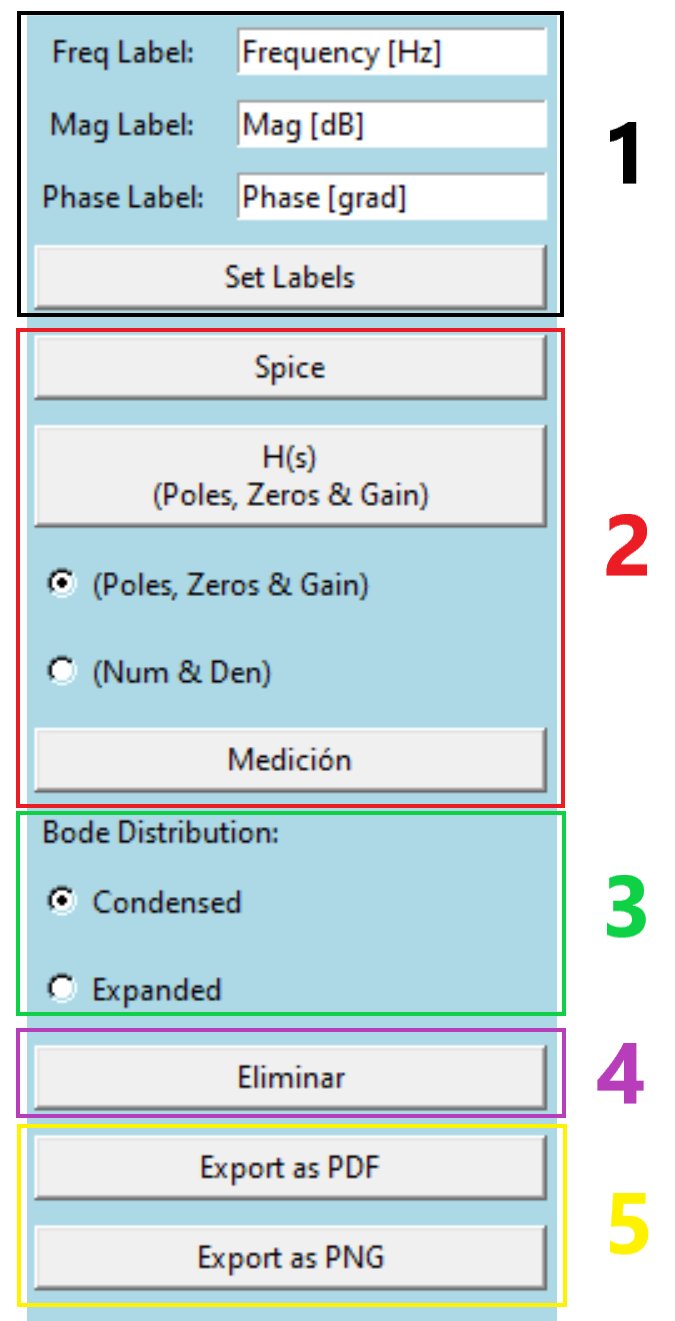
\includegraphics[scale=0.2]{controlPanel_ref.png}
\caption{Elementos del panel de controles con referencias}
\label{fig:controlPanel}
\end{figure}




\end{document}